\documentclass[11pt]{article}

% ---------------------------------------------------------------------------
% Embedding Compression for Dense Retrieval -- arXiv preprint
% Single-column, neutral preprint format. Compiles on TeX Live 2026 (latexmk).
% ---------------------------------------------------------------------------

\usepackage[utf8]{inputenc}
\usepackage[T1]{fontenc}
\usepackage[a4paper,margin=1in]{geometry}
\usepackage{amsmath,amssymb}
\usepackage{graphicx}
\graphicspath{{figures/}}
\usepackage{booktabs}
\usepackage{array}
\usepackage{multirow}
\usepackage{xcolor}
\usepackage{caption}
\captionsetup{font=small,labelfont=bf}
\usepackage{microtype}
\usepackage[numbers,sort&compress]{natbib}
\usepackage{authblk}
\usepackage[colorlinks=true,allcolors=blue!60!black]{hyperref}

% --- Title -----------------------------------------------------------------
% Alternative titles (pick one):
%  A) When Binarization Beats Full Precision: Effective Dimension and a
%     Controlled Study of Embedding Compression for Dense Retrieval
%  B) Compression as Regularization: Effective Dimension Explains When
%     Training-Time Binarization Helps Dense Retrieval
%  C) No Universal Winner: A Controlled Study of Embedding Compression
%     Across Retrieval Backbones
\title{\bfseries When Binarization Beats Full Precision:\\[2pt]
Effective Dimension and a Controlled Study of\\ Embedding Compression for Dense Retrieval}

% NOTE: confirm authorship and order with your advisor before posting.
\author[1]{Sajil Awale}
\author[1]{Simran KC}
\author[1]{Tathagata Mukherjee}
\affil[1]{Department of Computer Science, The University of Alabama in Huntsville (UAH), Huntsville, AL, USA}

\date{\today}

\begin{document}
\maketitle

\begin{abstract}
\noindent
Dense retrieval systems store one floating-point embedding per passage.
At billion-scale these indices dominate serving cost, because they must
reside in memory for low latency. Embedding compression reduces this cost.
However, the literature evaluates post-hoc and training-time methods on
different encoders and benchmarks, so practitioners cannot tell which to
use. We present a controlled comparison. Three encoders with different
retrieval priors (BGE, RoBERTa, and MPNet) are fine-tuned under identical
conditions. Each is compressed with post-hoc methods (INT8, binary,
Product Quantization (PQ), and TurboQuant), training-time
binarization-aware training (BAT) with two gradient surrogates
(Straight-Through Estimator and annealed tanh), Matryoshka Representation
Learning (MRL), and stacked combinations. All are evaluated on NanoBEIR.
We find that no method dominates across encoders. For BGE, which is
pre-trained for retrieval, post-hoc PQ leads the Pareto frontier at every
compression ratio. For RoBERTa and MPNet, training-time binarization leads
instead. Most surprisingly, BAT exceeds the full-precision baseline on
RoBERTa, raising Mean Reciprocal Rank at 10 (MRR@10) from 0.530 to 0.590.
We trace this to effective dimension. Binarization spreads embedding
variance across more axes, and the participation ratio rises from 11\% to
30\%. This improves ranking without changing recall, and the effect is
structural rather than a result of under-training. We release a
method-selection guide indexed by encoder and memory budget.\footnote{Code and
data: \url{https://github.com/AwaleSajil/Scaling-Embedding-Retrieval-Thesis}.
Interactive evaluation dashboard:
\url{https://huggingface.co/spaces/SajilAwale/Embedding-Compression-Eval}. Video
demo: \url{https://www.youtube.com/watch?v=2QgfmpQsKn8}.}
\end{abstract}

\section{Introduction}
\label{sec:intro}

Dense retrieval underpins many modern systems, including Retrieval-Augmented
Generation (RAG)~\citep{lewis2020retrieval}, question answering, and
semantic search~\citep{karpukhin2020dense, reimers2019sbert}. A bi-encoder
maps queries and passages to vectors, and relevance is scored by vector
similarity. Long documents are split into passages, so the indexed unit is a
passage that is encoded once and stored. These corpus vectors must reside in an
index in Random Access Memory (RAM) for low-latency
search~\citep{johnson2021billion, malkov2018efficient}. This memory is the dominant cost at scale. A single
BGE-base embedding is a 768-dimensional float32 vector of 3{,}072 bytes, so a
corpus of one billion passages needs roughly 2.9~TB of RAM for the embeddings
alone. Memory-optimized cloud instances are billed accordingly, so reducing
the index size translates directly into lower cost~\citep{aws2024pricing}.

Embedding compression addresses this cost, and two broad families exist.
\emph{Post-hoc} methods compress a fixed embedding after training: scalar
quantization to INT8, binary quantization with Hamming
search~\citep{shakir2024embedding}, Product Quantization
(PQ)~\citep{jegou2010product}, and recent oblivious quantizers such as
TurboQuant~\citep{zandieh2025turboquant}. \emph{Training-time} methods bake
the compression into the objective: binarization-aware training through a
Straight-Through Estimator (STE)~\citep{bengio2013estimating, courbariaux2016bnn}
or an annealed tanh surrogate~\citep{yamada2021efficient}, and Matryoshka
Representation Learning (MRL)~\citep{kusupati2022matryoshka}, which front-loads
information so that truncated prefixes remain usable.

\paragraph{The gap.}
Despite a rich set of methods, a practitioner cannot easily decide which to
use. The reason is methodological: post-hoc and training-time methods are
studied on different encoders, with different training data and benchmarks, and
they rarely meet on common ground. The broadest post-hoc
comparison~\citep{correct2025} does vary the backbone, but omits training-time
methods, while the training-time studies~\citep{qama2025, yamada2021efficient}
fix a single backbone or a narrow pair. So it is unknown whether the best method
depends on the encoder's retrieval prior, and whether training-time compression
is worth its added cost relative to a simple post-hoc transform.

\paragraph{This work.}
We run a controlled comparison. Three encoders with deliberately different
retrieval priors, BGE~\citep{xiao2023c}, RoBERTa~\citep{liu2019roberta}, and
MPNet~\citep{song2020mpnet}, are fine-tuned under identical conditions on the
same data. Each is then compressed by every method above and by stacked
combinations, and all are evaluated on NanoBEIR~\citep{nanobeir2024} with
paired significance testing. Because the only variable that changes is the
compression method (and the backbone), differences are attributable to the
method rather than to confounds of data or benchmark.

\paragraph{Findings.}
The headline result is that no single method dominates, and the winner depends
on the encoder. For BGE, which is pre-trained at scale with a contrastive
retrieval objective, post-hoc PQ leads the Pareto frontier at every tested
compression ratio. For RoBERTa and MPNet, which lack retrieval pre-training,
training-time binarization leads instead. Most surprisingly, binarization-aware
training \emph{exceeds the full-precision baseline} on RoBERTa, raising Mean Reciprocal Rank at 10 (MRR@10)
from 0.530 to 0.590, even though binarization removes information.

We explain this with the geometry of the embedding space. Encoders without
retrieval pre-training produce anisotropic embeddings that occupy a narrow
cone~\citep{ethayarajh2019contextual}, which saturates similarities and harms
fine-grained ranking. We quantify this with the \emph{effective dimension}, or
participation ratio~\citep{litwinkumar2017optimal, gao2017theory}.
Binarization-aware training spreads variance across more axes, raising the
participation ratio from 11\% to 30\% of 768 dimensions for RoBERTa. The gain
shows up in ranking, not coverage: MRR@10 improves while Recall@10 remains
unchanged.
The effect is present from the first checkpoint and does not close with more
training, so it is structural rather than a symptom of under-training. Because
ranking under this metric depends on angular separation rather than per-axis
precision, one bit per dimension is sufficient to realize the benefit.

\paragraph{Contributions.}
\begin{itemize}
  \item A controlled, cross-encoder comparison of post-hoc, training-time, and
        stacked embedding compression for dense retrieval, reported as Pareto
        frontiers with paired significance tests
        (Sections~\ref{sec:method} and~\ref{sec:results}).
  \item The finding that binarization-aware training can exceed full precision
        on encoders without retrieval pre-training, with a mechanism:
        binarization raises the effective dimension of the embedding space and
        improves ranking without changing recall
        (Section~\ref{sec:results}, Section~\ref{sec:discussion}).
  \item Evidence that the best gradient surrogate and the value of stacking are
        backbone-dependent, including that annealed tanh combines with MRL more
        cleanly than STE, and that MRL$+$PQ extends the frontier to high
        compression (Section~\ref{sec:results}).
  \item A practical method-selection guide indexed by encoder type and memory
        budget (Section~\ref{sec:discussion}), released together with all code
        and an interactive evaluation dashboard for browsing the full results.

\end{itemize}

\section{Related Work}
\label{sec:related}

Embedding compression splits into two families by \emph{when} the compression
happens. Post-hoc methods act on a frozen embedding. Training-time methods build
the compression into the objective. We review each, then position our study
against the four closest works.

\paragraph{Post-hoc compression.}
The simplest compressors transform an embedding after training, so they are cheap
and model-agnostic. Scalar quantization maps float32 to INT8 with per-dimension
calibration and is near-lossless at $4\times$~\citep{shakir2024embedding}. Binary
quantization keeps only the sign of each dimension and searches in Hamming space
at $32\times$. PQ~\citep{jegou2010product} splits the
vector into subspaces and encodes each with a learned codebook, and it remains
the strong learning-to-hash baseline. TurboQuant~\citep{zandieh2025turboquant}
is a recent data-oblivious quantizer that applies a random rotation before
scalar quantization to approach optimal distortion. The common limitation is
that none of these methods can change the representation they are handed.

\paragraph{Training-time compression.}
A second family reshapes the representation during training, at the cost of a
training run. Binarization is not differentiable, so it needs a gradient
surrogate. The STE~\citep{bengio2013estimating,
courbariaux2016bnn} passes gradients through the sign unchanged, while an annealed
tanh sharpens a smooth surrogate into a step function over
training~\citep{yamada2021efficient, yang2019quantization, schrodter2025trainable}.
MRL~\citep{kusupati2022matryoshka} takes a
different route and trains nested sub-vectors, so one model serves many truncation
dimensions. These methods can fix geometry that post-hoc methods cannot, but they
have mostly been studied one at a time.

\paragraph{The closest work falls in two camps.}
On the \emph{evaluation} side, CoRECT~\citep{correct2025} is nearest to us. It
compares compression techniques across corpus size and compression ratio for
several models, but only for post-hoc methods, so training-time compression is
absent. On the \emph{method} side, QAMA~\citep{qama2025} is nearest. It stacks
MRL with multi-bit quantization-aware training and learned thresholds, but it
relies on a penalty loss rather than a differentiable surrogate, and it never
compares gradient surrogates. Two more works touch single pieces of our study.
The Binary Passage Retriever (BPR)~\citep{yamada2021efficient} compares annealed
tanh against PQ and full precision, but never against STE. BEBR~\citep{gan2023binary}
deploys recurrent residual binarization at scale with runtime-selectable bit
depth, but trains the compressor separately from the encoder. Our own prior work
on a scientific-domain encoder~\citep{pantha2026indussde} shows that
binarization-aware training beats post-hoc binary, but on a single model, a single
domain, and STE alone.

\paragraph{Our position.}
No prior work compares post-hoc, training-time, \emph{and} stacked compression on
common ground. The broadest evaluation, CoRECT, varies the backbone but covers
only post-hoc methods; the training-time studies fix a single backbone or a
narrow pair. As a result, whether the best compression method depends on the
encoder's retrieval prior has not been tested, and the backbone-dependent
behavior we report has not been explained. We close that gap, and we connect the
behavior to the anisotropy of contextual
embeddings~\citep{ethayarajh2019contextual} through the effective
dimension~\citep{litwinkumar2017optimal, gao2017theory}.

\section{Experimental Design}
\label{sec:method}

Our design is built to isolate the effect of the compression method. We hold the
training data, schedule, and benchmark fixed, and we vary only two things: the
encoder backbone and the compression method. Any difference we report is
therefore attributable to one of those two factors, not to a confound of data or
tuning.

\subsection{Backbones}
\label{subsec:backbones}
We choose three 768-dimensional encoders that differ in how much retrieval prior
they carry. BGE-base-en-v1.5~\citep{xiao2023c} is pre-trained at scale with a
contrastive retrieval objective and has the strongest prior. RoBERTa-base~\citep{liu2019roberta}
is pre-trained with masked language modeling alone and has the weakest retrieval
geometry. MPNet-base~\citep{song2020mpnet} sits between the two. All three are
fine-tuned as bi-encoders~\citep{reimers2019sbert} with mean pooling and cosine
similarity, so the only prior difference is the one we want to study.

\subsection{Training}
\label{subsec:training}
Each backbone is fine-tuned with a Multiple Negatives Ranking Loss
(MNRL)~\citep{oord2018representation}, which pulls a query toward its positive
passage and pushes it away from the in-batch negatives. The training mixture
combines seven public retrieval sources~\citep{bajaj2016ms, lo2020s2orc,
kwiatkowski2019natural, joshi2017triviaqa, yang2018hotpotqa, gao2021simcse},
sampled with weights that rebalance the mixture so no single source dominates.
Crucially, every backbone and every training-time variant uses the same
hyperparameter configuration (Appendix~\ref{app:hyperparams}), so no result is an
artifact of per-method tuning. Training is data-parallel across four GPUs.

\subsection{Compression methods}
\label{subsec:methods}
We evaluate four post-hoc methods, two training-time binarization variants, MRL,
and stacked combinations of the two axes.

\paragraph{Post-hoc.}
We apply INT8 scalar quantization at $4\times$; binary quantization with Hamming
search at $32\times$; PQ~\citep{jegou2010product} over a grid of subspace counts
$M$ and code widths $n \in \{4,8\}$, spanning $32\times$ to $384\times$; and
TurboQuant~\citep{zandieh2025turboquant} at $1$ to $8$ bits per dimension,
spanning $4\times$ to $32\times$. Because all post-hoc transforms read from a
single cached float32 encoding per checkpoint, they add no encoding cost.

\paragraph{Training-time.}
Binarization-aware training (BAT) inserts a binary layer before the loss and
trains it with one of two gradient surrogates: STE~\citep{bengio2013estimating}
or annealed tanh at rate $\gamma=0.1$~\citep{yamada2021efficient}. Both produce
768-bit codes at inference, for $32\times$ compression. MRL~\citep{kusupati2022matryoshka}
instead trains nested sub-vectors, which we evaluate at
$d \in \{32,64,128,256,512,768\}$.

\paragraph{Stacked.}
We then pair MRL truncation with a second compressor along the precision axis.
This gives pure training-time stacks (MRL$+$BAT-STE, MRL$+$BAT-atanh) and hybrid
stacks (MRL$+$post-hoc-binary, MRL$+$TurboQuant, MRL$+$PQ), which together reach
$384\times$ and beyond.

\subsection{Evaluation}
\label{subsec:eval}
We evaluate on NanoBEIR~\citep{nanobeir2024}, an efficient proxy for
BEIR~\citep{thakur2021beir} with 13 subsets, 649 queries, and 57{,}390 corpus
documents. The primary metric is MRR@10, macro-averaged over the 13 subsets; we
also report Recall@10 and normalized Discounted Cumulative Gain at 10
(nDCG@10)~\citep{jarvelin2002cumulated}. Float32 encodings are cached once per
checkpoint, and every transform is applied at load time, so methods that share a
checkpoint also share one encoding. To decide whether a gap between two methods
is real, we use a paired Wilcoxon signed-rank test on per-query
MRR@10~\citep{wilcoxon1945individual} at $\alpha=0.05$. We report compression as
the ratio of float32 index bytes to compressed index bytes, and we read off
Pareto frontiers in the quality-compression plane.

\section{Results}
\label{sec:results}

\subsection{Float32 baselines}
\label{subsec:baselines}
Table~\ref{tab:baselines} reports the float32 ceilings. Fine-tuning helps the
general-purpose encoders dramatically (RoBERTa $+0.434$, MPNet $+0.426$) but
leaves BGE essentially unchanged ($-0.006$, not significant, paired Wilcoxon
$p=0.49$), because BGE is already pre-trained for retrieval. These scores are
the upper bounds for every compression method.

\begin{table}[t]
  \centering
  \caption{Float32 baselines: pre-trained vs fine-tuned, mean MRR@10 over 13
  NanoBEIR subsets. $\Delta$ is the change from fine-tuning.}
  \label{tab:baselines}
  \begin{tabular}{lccc}
    \toprule
    \textbf{Configuration} & \textbf{BGE} & \textbf{RoBERTa} & \textbf{MPNet} \\
    \midrule
    Pre-trained  & 0.691 & 0.097 & 0.156 \\
    Fine-tuned   & 0.685 & 0.530 & 0.582 \\
    $\Delta$     & $-0.006$ & $+0.434$ & $+0.426$ \\
    \bottomrule
  \end{tabular}
\end{table}

\subsection{Post-hoc compression}
\label{subsec:posthoc}
INT8 at $4\times$ is near-lossless on all backbones (largest drop $-0.015$ on
MPNet; full INT8 and TurboQuant tables in Appendix~\ref{app:posthoc}). At
$32\times$, the four post-hoc methods separate clearly
(Table~\ref{tab:posthoc32}, Figure~\ref{fig:crossmethod}). The ordering
PQ $>$ TurboQuant-1bit $>$ post-hoc binary is stable across backbones, and PQ
with $8$-bit codes is best for BGE and MPNet, recovering all but $0.6$ points of
the BGE float32 ceiling. Post-hoc binary is the weakest method everywhere.

\begin{table}[t]
  \centering
  \caption{Four post-hoc methods at $32\times$, mean MRR@10. Best per backbone
  in bold; ties at displayed precision bolded together.}
  \label{tab:posthoc32}
  \begin{tabular}{lcccc}
    \toprule
    \textbf{Method} & \textbf{Ratio} & \textbf{BGE} & \textbf{RoBERTa} & \textbf{MPNet} \\
    \midrule
    Float32 (fine-tuned)         & $1\times$  & 0.685 & 0.530 & 0.582 \\
    Post-hoc binary              & $32\times$ & 0.646 & 0.501 & 0.534 \\
    TurboQuant, 1-bit            & $32\times$ & 0.666 & \textbf{0.519} & 0.547 \\
    PQ ($M{=}192, n{=}4$)        & $32\times$ & 0.675 & \textbf{0.519} & 0.549 \\
    PQ ($M{=}96, n{=}8$)         & $32\times$ & \textbf{0.679} & 0.514 & \textbf{0.562} \\
    \bottomrule
  \end{tabular}
\end{table}

\begin{figure}[t]
  \centering
  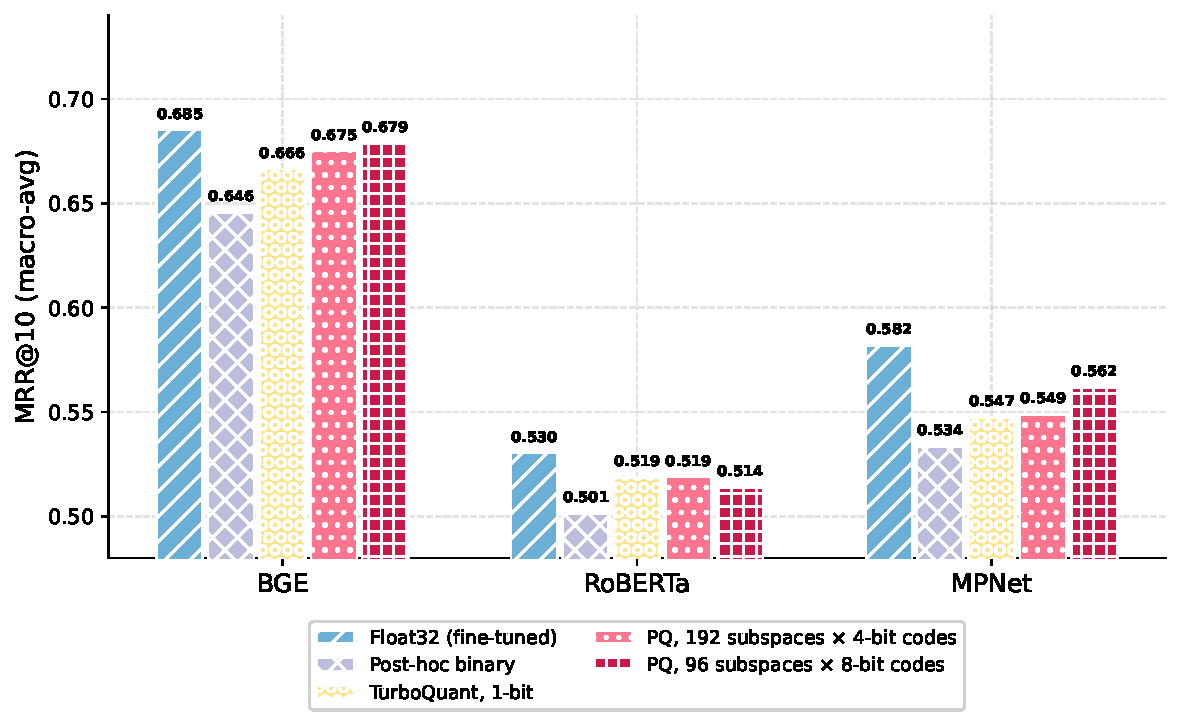
\includegraphics[width=0.8\textwidth]{fig_crossmethod_32x.pdf}
  \caption{Post-hoc methods at $32\times$, mean MRR@10 by backbone. The $y$-axis
  starts at 0.48 to highlight inter-method differences.}
  \label{fig:crossmethod}
\end{figure}

\subsection{Training-time binarization beats post-hoc, and sometimes float32}
\label{subsec:bat}
Both BAT variants beat post-hoc binary on every backbone
(Table~\ref{tab:bat}). The gains are largest on the general-purpose encoders:
BAT-STE improves over post-hoc binary by $6.4$ points on RoBERTa and $4.8$ on
MPNet, versus $1.3$ on BGE. Strikingly, BAT \emph{exceeds the float32 ceiling}
on RoBERTa: BAT-STE reaches 0.565 ($p=0.005$) and BAT-atanh reaches 0.590
($p<10^{-3}$), against a float32 baseline of 0.530. BAT-STE matches float32 on
MPNet and BAT-STE is best on BGE, so the best surrogate is backbone-dependent.

\begin{table}[t]
  \centering
  \caption{Binarization-aware training vs post-hoc binary at $32\times$, mean
  MRR@10. The float32 fine-tune is the ceiling. Best $32\times$ result per
  backbone in bold.}
  \label{tab:bat}
  \begin{tabular}{lcccc}
    \toprule
    \textbf{Method} & \textbf{Ratio} & \textbf{BGE} & \textbf{RoBERTa} & \textbf{MPNet} \\
    \midrule
    Float32 (ceiling)        & $1\times$  & 0.685 & 0.530 & 0.582 \\
    Post-hoc binary          & $32\times$ & 0.646 & 0.501 & 0.534 \\
    BAT-STE                  & $32\times$ & \textbf{0.658} & 0.565 & \textbf{0.582} \\
    BAT-atanh ($\gamma{=}0.1$) & $32\times$ & 0.638 & \textbf{0.590} & 0.580 \\
    \bottomrule
  \end{tabular}
\end{table}

\subsection{Why binarization beats full precision on RoBERTa}
\label{subsec:effdim}
The result is counterintuitive, because binarization removes information. We
analyze it in three steps.

\paragraph{The gain is in ranking, not coverage.}
On RoBERTa, MRR@10 rises from 0.530 to 0.565 (STE) and 0.590 (atanh), both
significant (Wilcoxon $p=0.005$ and $p<0.001$; all tests in
Appendix~\ref{app:sig}). Recall@10 barely moves (0.553 to
0.552 and 0.560) and is not significant ($p=0.57$, $p=0.27$). So the same
relevant documents are retrieved, but the correct answers are ranked higher.

\paragraph{The mechanism is effective dimension.}
Encoders without retrieval pre-training produce anisotropic embeddings that
occupy a narrow cone~\citep{ethayarajh2019contextual}. We measure this with the
effective dimension, or participation ratio~\citep{litwinkumar2017optimal,
gao2017theory},
\begin{equation}
  d_{\mathrm{eff}} = \frac{\left(\sum_i \lambda_i\right)^2}{\sum_i \lambda_i^2},
\end{equation}
where $\lambda_i$ are the 768 eigenvalues of the centered embedding covariance.
$d_{\mathrm{eff}}$ counts how many axes carry variance. Float32 RoBERTa is the
most compressed of the three spaces ($d_{\mathrm{eff}}=85$, or 11.0\% of 768).
Binarization-aware training spreads variance across more axes, raising
$d_{\mathrm{eff}}$ to 25.7\% (STE) and 30.0\% (atanh), and MRR@10 tracks this
increase (Table~\ref{tab:effdim}, Figure~\ref{fig:effdim}). Because ranking
under Hamming and cosine depends on angular separation rather than per-axis
precision, one bit per dimension is enough to realize the benefit.

\begin{table}[t]
  \centering
  \caption{Effective dimension $d_{\mathrm{eff}}$ (participation ratio) with
  retrieval quality, on the pooled NanoBEIR corpus. Binarization-aware training
  raises both $d_{\mathrm{eff}}$ and MRR@10 for RoBERTa.}
  \label{tab:effdim}
  \begin{tabular}{lcccc}
    \toprule
    \textbf{Model} & $d_{\mathrm{eff}}$ & \textbf{\% of 768} & \textbf{MRR@10} & \textbf{Recall@10} \\
    \midrule
    RoBERTa-FT        & 85  & 11.0\% & 0.530 & 0.553 \\
    BGE-FT            & 135 & 17.6\% & 0.685 & 0.656 \\
    MPNet-FT          & 102 & 13.3\% & 0.582 & 0.583 \\
    RoBERTa-BAT-STE   & 197 & 25.7\% & 0.565 & 0.552 \\
    RoBERTa-BAT-atanh & 230 & 30.0\% & \textbf{0.590} & 0.560 \\
    \bottomrule
  \end{tabular}
\end{table}

\begin{figure}[t]
  \centering
  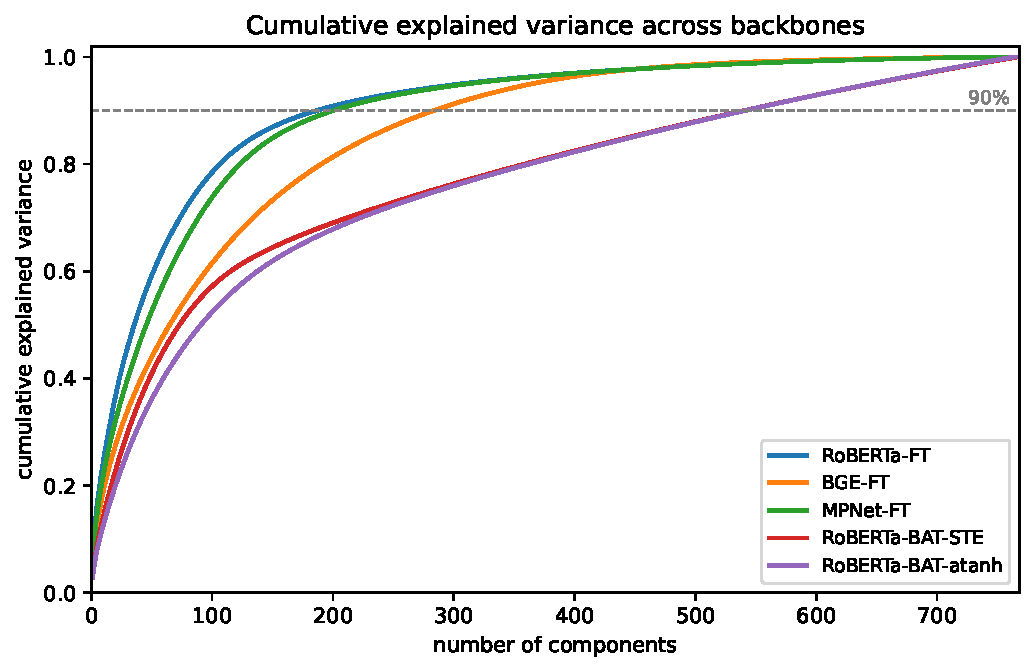
\includegraphics[width=0.78\textwidth]{fig_roberta_effdim.pdf}
  \caption{Cumulative explained variance vs number of principal components. A
  curve that rises quickly indicates a low effective dimension. RoBERTa-FT rises
  fastest; RoBERTa-BAT-atanh rises slowest.}
  \label{fig:effdim}
\end{figure}

\paragraph{It is RoBERTa-specific, and structural.}
BGE already has the highest float32 $d_{\mathrm{eff}}$ (17.6\%), so it has little
anisotropy to correct and binarization only costs it quality. MPNet is in
between and is near-lossless under BAT. RoBERTa has the most to gain because it
starts most compressed, which gives the relative ordering RoBERTa $>$ MPNet $>$
BGE. The gain is not under-training: evaluating intermediate checkpoints every
2{,}000 steps (Figure~\ref{fig:trajectory}), both BAT variants sit above the
float32 fine-tune from the first checkpoint, and the gap does not close with
more training.

\begin{figure}[t]
  \centering
  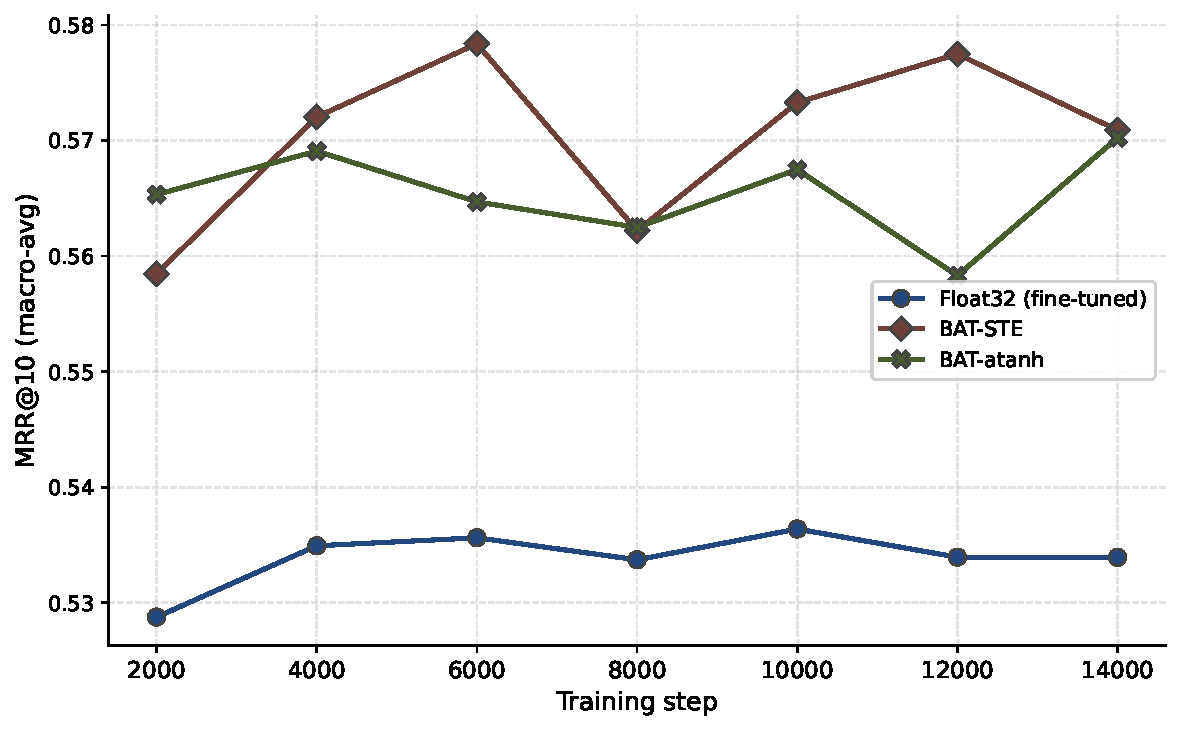
\includegraphics[width=0.78\textwidth]{fig_training_trajectory.pdf}
  \caption{Mean MRR@10 at intermediate RoBERTa checkpoints. The gap from BAT to
  the float32 fine-tune is present early and does not close with training.}
  \label{fig:trajectory}
\end{figure}

\subsection{Matryoshka and stacked compression}
\label{subsec:stacked}
MRL alone is near-lossless to $d=256$ ($3\times$) on all backbones, then drops
sharply below $d=128$ (Figure~\ref{fig:mrl}; full table in
Appendix~\ref{app:mrl}). Its value is that it composes with
a second compressor. Stacking MRL with a precision-reduction method pushes the
frontier well beyond what either axis reaches alone
(Figure~\ref{fig:stacked}). Three results stand out. First, MRL$+$PQ dominates
the high-compression region: at $\geq 96\times$ it is best on every backbone,
and its margin grows with compression (at $384\times$, by 13.0, 6.2, and 7.5
points on BGE, RoBERTa, and MPNet). Second, MRL$+$BAT-atanh beats MRL$+$BAT-STE
on all backbones and all compression ratios, unlike the standalone case where
atanh wins only on RoBERTa; binarizing with a sign before the MRL loss destroys
more magnitude information than tanh. Third, MRL$+$BAT-atanh crosses the float32
ceiling on RoBERTa at $32\times$ (0.560 vs 0.530), the only backbone for which
any stacked configuration does so.

\begin{figure}[t]
  \centering
  
\includegraphics[width=0.78\textwidth]{fig_mrl_truncation.pdf}
  \caption{Mean MRR@10 vs MRL truncation dimension $d$. The point at $d=768$ is
  the float32 baseline.}
  \label{fig:mrl}
\end{figure}

\begin{figure}[t]
  \centering
  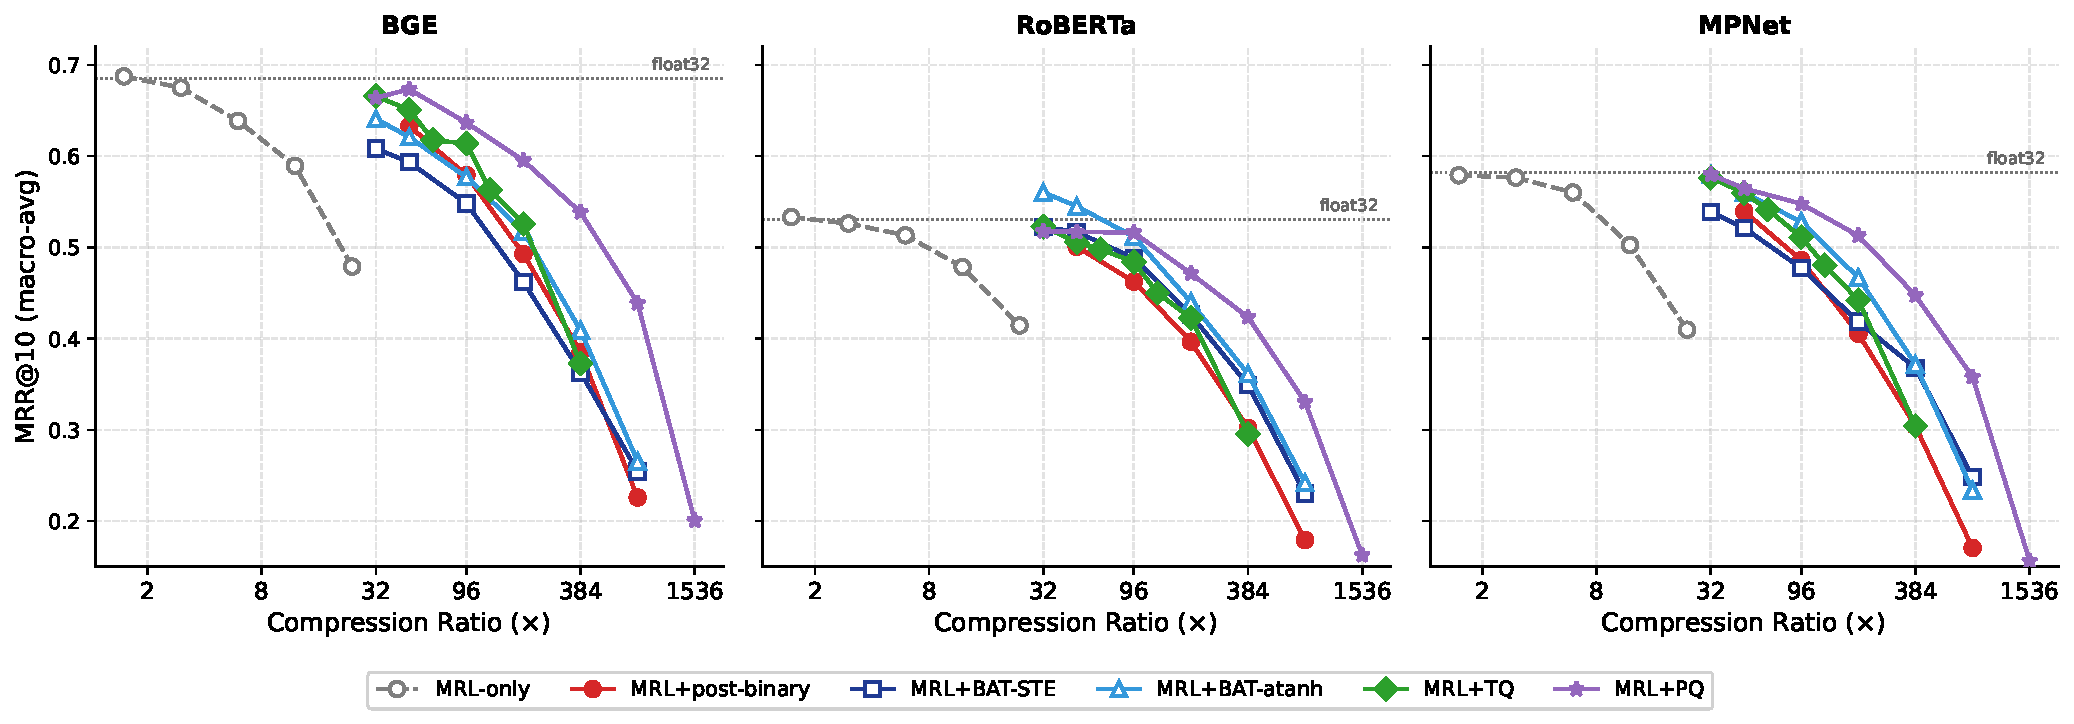
\includegraphics[width=\textwidth]{fig_stacked_combinations.pdf}
  \caption{Mean MRR@10 vs compression ratio for the five stacked combinations
  and MRL-only (grey dashed). Hollow markers are pure training-time stacks;
  filled markers are hybrid stacks. The dotted line is the float32 baseline.}
  \label{fig:stacked}
\end{figure}

\subsection{Pareto frontiers and cross-backbone generalization}
\label{subsec:pareto}

\paragraph{The Pareto frontier looks different for each backbone.}
Figure~\ref{fig:pareto} plots every configuration as a per-backbone Pareto
frontier of quality against compression. For BGE, no training-time method reaches
the frontier at all. It runs through TurboQuant at moderate ratios, then PQ and
stacked MRL$+$PQ from $32\times$ out past $1500\times$
(Appendix~\ref{app:pareto}). For RoBERTa and MPNet the picture flips: the best
$32\times$ point is a \emph{training-time} method. BAT-atanh leads on RoBERTa
(0.590, 7.1 points above the best post-hoc option), and BAT-STE leads on MPNet
(0.582, 2.0 points above).

\paragraph{The best method does not transfer across backbones.}
To compare backbones of different quality fairly, we divide each score by its own
backbone's float32 score (Figure~\ref{fig:crossbackbone}). The post-hoc methods
keep a similar fraction of quality on all three backbones, so they generalize.
The training-time methods do not: BAT-STE and BAT-atanh help most on RoBERTa,
less on MPNet, and least on BGE. The practical lesson is simple. A study run only on BGE would pick post-hoc PQ
as the best method at $32\times$. But on general-purpose backbones,
training-time binarization is the better choice at $32\times$. So results from
one backbone do not always transfer to another.

\begin{figure}[t]
  \centering
  
\includegraphics[width=\textwidth]{fig_pareto.pdf}
  \caption{Quality vs compression Pareto frontiers for BGE, RoBERTa, and MPNet
  ($x$-axis log scale). Filled markers are Pareto-optimal; hollow markers are
  dominated. Colour encodes method family.}
  \label{fig:pareto}
\end{figure}

\begin{figure}[t]
  \centering
  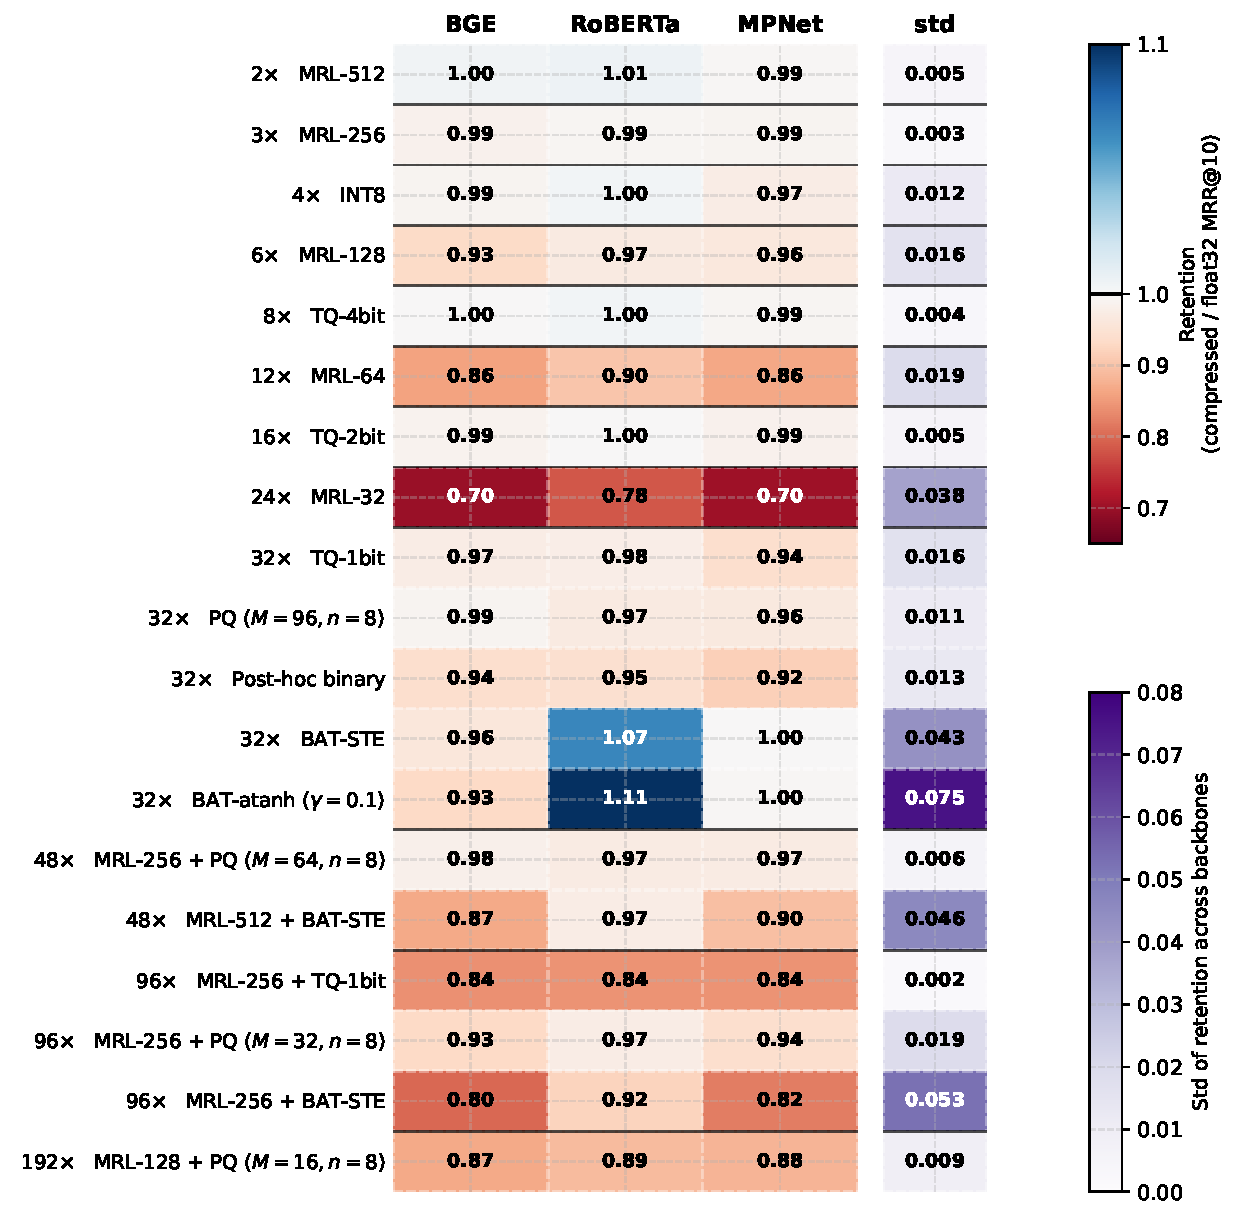
\includegraphics[width=0.95\textwidth]{fig_cross_backbone.pdf}
  \caption{Quality retention (compressed MRR@10 divided by the same backbone's
  float32 MRR@10) by configuration. The rightmost column shows the
  cross-backbone standard deviation.}
  \label{fig:crossbackbone}
\end{figure}

\section{Discussion}
\label{sec:discussion}

\paragraph{Binary constraints as a regularizer.}
The central finding reframes binarization. On an encoder without retrieval
pre-training, a sign constraint is not only a compression step but a regularizer
that de-anisotropizes the embedding space. It spreads variance across more axes,
de-saturates the similarity distribution, and improves fine-grained ranking. The
constraint helps most where the float32 space is most anisotropic, which is why
the benefit is ordered RoBERTa $>$ MPNet $>$ BGE and is absent for the
retrieval-pre-trained encoder. The effective dimension is thus a cheap
\emph{diagnostic}: measuring $d_{\mathrm{eff}}$ of an encoder's float32
embeddings, which costs one eigendecomposition and no training, predicts whether
training-time binarization will help or hurt that backbone.

\paragraph{A method-selection guide.}
Because no method dominates, the practical contribution is a rule indexed by two
variables: whether the encoder is pre-trained for retrieval, and the target
memory budget (Table~\ref{tab:cheatsheet}).

\begin{table}[t]
  \centering
  \caption{Recommended compression method by encoder type and compression
  budget, from the Pareto frontiers in Section~\ref{subsec:pareto}.}
  \label{tab:cheatsheet}
  \begin{tabular}{lll}
    \toprule
    \textbf{Budget} & \textbf{Retrieval-pre-trained (BGE)} & \textbf{General-purpose (RoBERTa, MPNet)} \\
    \midrule
    $\leq 8\times$        & INT8 or TurboQuant-4bit (near-lossless) & INT8 or TurboQuant-4bit (near-lossless) \\
    $32\times$            & Post-hoc PQ ($n{=}8$)                   & Training-time BAT (atanh or STE) \\
    $\geq 96\times$       & Stacked MRL$+$PQ                        & Stacked MRL$+$PQ \\
    \bottomrule
  \end{tabular}
\end{table}

\paragraph{Threats to validity.}
We state the limitations plainly. First, evaluation is on NanoBEIR, whose
subsets are small; the backbone-dependent conclusions should be confirmed on
full BEIR~\citep{thakur2021beir} or MTEB~\citep{muennighoff2022mteb} at larger
corpus scale, where compression behavior can shift. Second, each model is
fine-tuned for a single epoch; although the training-trajectory analysis
(Section~\ref{subsec:effdim}) rules out under-training as the cause of the BAT
gain, longer schedules could change absolute scores. Third, we report
compression ratios rather than measured query latency and on-disk index size;
these would close the loop from memory savings to end-to-end cost. Finally, the
effective-dimension account is correlational across five models; a controlled
intervention, such as injecting anisotropy into BGE and observing whether BAT's
relative benefit rises, would strengthen the causal claim.

\section{Conclusion}
\label{sec:conclusion}

We compared post-hoc, training-time, and stacked embedding compression for dense
retrieval on common ground, across three encoders with different retrieval
priors. No single method dominates. The right choice depends on whether the
encoder is pre-trained for retrieval and on the memory budget: post-hoc PQ leads
for the retrieval-pre-trained encoder, while training-time binarization leads for
the general-purpose encoders, and stacked MRL$+$PQ leads at high compression for
all. The most surprising result is that binarization-aware training can exceed
the full-precision baseline on an encoder without retrieval pre-training. We
explained this through effective dimension: binarization spreads embedding
variance across more axes, improving ranking without changing recall, and the
effect is structural rather than a symptom of under-training.

Future work follows directly. Scaling the evaluation to full BEIR and MTEB, and
adding measured latency and index size, would test whether the backbone-dependent
frontiers hold at deployment scale. Pairing MRL with recurrent residual
binarization~\citep{gan2023binary} would give runtime-selectable dimension and
bit depth. And a controlled anisotropy intervention would turn the
effective-dimension correlation into a causal account of when compression helps
retrieval.


\bibliographystyle{plainnat}
\bibliography{ref}

\clearpage
\appendix

\section{Training Details and Hyperparameters}
\label{app:hyperparams}
All three backbones and all six training-time variants share the single
configuration in Table~\ref{tab:hyperparams}, so reported differences are not an
artifact of per-method tuning. Training uses multi-GPU data-parallelism across
four GPUs; the effective batch size is the product of the per-device batch,
gradient accumulation, and device count.

\begin{table}[h]
  \centering
  \caption{Shared training configuration.}
  \label{tab:hyperparams}
  \begin{tabular}{ll}
    \toprule
    \textbf{Setting} & \textbf{Value} \\
    \midrule
    Base encoders & BGE-base-en-v1.5, RoBERTa-base, MPNet-base \\
    Max sequence length & 512 \\
    Pooling & Mean \\
    Loss & Multiple Negatives Ranking Loss (cosine) \\
    Optimizer & AdamW \\
    Learning rate & $2\times10^{-5}$ \\
    LR schedule & Linear, warmup ratio 0.1 \\
    Weight decay & 0.1 \\
    Per-device batch size & 16 \\
    Gradient accumulation & 8 \\
    Data-parallel devices & 4 \\
    Effective batch size & 512 \\
    Epochs & 1 \\ % TODO: config.yaml sets num_train_epochs=2; confirm against the actual runs.
    Eval/checkpoint interval & every 2{,}000 steps \\
    MRL truncation dims & $\{32, 64, 128, 256, 512, 768\}$ \\
    Annealed tanh rate $\gamma$ & 0.1 \\
    \bottomrule
  \end{tabular}
\end{table}

\section{Training Data and Benchmark Composition}
\label{app:data}

\paragraph{Training mixture.}
The training mixture draws from seven public sources spanning passage retrieval,
title-to-abstract prediction, duplicate-question detection, natural language
inference, and open-domain question answering (Table~\ref{tab:datamix}). A
weighted batch sampler controls each source's contribution: the effective number
of examples from a source is proportional to its weight times its size. Weights
below one downsample the two largest, weakly retrieval-specific sources (S2ORC
and MS MARCO), while weights above one oversample the smaller question-answering
sources (Natural Questions, TriviaQA, HotpotQA). This reduces the raw 58.73M
examples to an effective mixture of about 4.19M per epoch, which preserves source
diversity while cutting training time.

\begin{table}[h]
  \centering
  \caption{Training data mixture. Effective rows are each source's approximate
  contribution after weighted sampling (proportional to weight $\times$ total
  rows), scaled so the mixture totals about 4.19M examples per epoch.}
  \label{tab:datamix}
  \resizebox{\textwidth}{!}{%
  \begin{tabular}{llrrr}
    \toprule
    \textbf{Source} & \textbf{Pair type} & \textbf{Total rows} & \textbf{Weight} & \textbf{Effective rows} \\
    \midrule
    MS MARCO~\citep{bajaj2016ms}                     & Query to passage (triplet)         & 13.64M & 0.15 & 1.94M \\
    S2ORC~\citep{lo2020s2orc}                        & Title to abstract (pair)           & 41.77M & 0.01 & 0.40M \\
    Quora duplicates                                 & Duplicate question (triplet)       & 2.79M  & 0.15 & 0.40M \\
    NLI for SimCSE~\citep{gao2021simcse}             & Entailment/contradiction (triplet) & 0.27M  & 2    & 0.52M \\
    Natural Questions~\citep{kwiatkowski2019natural} & Question to answer (pair)          & 0.10M  & 4    & 0.38M \\
    TriviaQA~\citep{joshi2017triviaqa}               & Question to answer (triplet)       & 0.06M  & 4    & 0.23M \\
    HotpotQA~\citep{yang2018hotpotqa}                & Multi-hop question to answer (triplet) & 0.08M & 4 & 0.32M \\
    \midrule
    \textbf{Total} & & \textbf{58.73M} & & \textbf{$\sim$4.19M} \\
    \bottomrule
  \end{tabular}}
\end{table}

\paragraph{Evaluation benchmark.}
NanoBEIR~\citep{nanobeir2024} is a lightweight subset of
BEIR~\citep{thakur2021beir}, built by sampling each BEIR subset down to 50
queries and a small corpus. We use all 13 subsets: ArguAna, ClimateFEVER,
DBPedia, FEVER, FiQA2018, HotpotQA, MSMARCO, NFCorpus, NQ, QuoraRetrieval,
SCIDOCS, SciFact, and Touch\'e2020. Each subset has 50 queries (49 for
Touch\'e2020) and a corpus of between 2{,}260 and 6{,}100 passages, totaling 649
queries and 57{,}390 corpus passages. Table~\ref{tab:nanobeir} gives the
per-subset breakdown.

\begin{table}[h]
  \centering
  \caption{NanoBEIR evaluation subsets. All subsets have 50 queries except
  Touch\'e2020 (49), with corpora of 2{,}260 to 6{,}100 passages, totaling 649
  queries and 57{,}390 passages.}
  \label{tab:nanobeir}
  \resizebox{\textwidth}{!}{%
  \begin{tabular}{llrrl}
    \toprule
    \textbf{\#} & \textbf{Subset} & \textbf{Queries} & \textbf{Corpus} & \textbf{Task (query to document)} \\
    \midrule
    1  & NanoArguAna        & 50 & 3{,}690 & Counter-argument retrieval (claim to argument) \\
    2  & NanoClimateFEVER   & 50 & 3{,}460 & Fact-checking (claim to document) \\
    3  & NanoDBPedia        & 50 & 6{,}100 & Entity retrieval (query to document) \\
    4  & NanoFEVER          & 50 & 5{,}050 & Fact-checking (claim to document) \\
    5  & NanoFiQA2018       & 50 & 4{,}650 & Financial question answering (question to document) \\
    6  & NanoHotpotQA       & 50 & 5{,}140 & Multi-hop question answering (question to document) \\
    7  & NanoMSMARCO        & 50 & 5{,}090 & Web search / general QA (question to passage) \\
    8  & NanoNFCorpus       & 50 & 3{,}000 & Biomedical retrieval (query to document) \\
    9  & NanoNQ             & 50 & 5{,}090 & Open-domain question answering (question to document) \\
    10 & NanoQuoraRetrieval & 50 & 5{,}100 & Duplicate detection (question to question) \\
    11 & NanoSCIDOCS        & 50 & 2{,}260 & Citation prediction (title to document) \\
    12 & NanoSciFact        & 50 & 2{,}970 & Scientific fact-checking (claim to document) \\
    13 & NanoTouche2020     & 49 & 5{,}790 & Conversational argument retrieval (question to argument) \\
    \midrule
    \multicolumn{2}{l}{\textbf{Total}} & \textbf{649} & \textbf{57{,}390} & \\
    \bottomrule
  \end{tabular}}
\end{table}

\section{Full Post-hoc Results}
\label{app:posthoc}
Tables~\ref{tab:int8full} and~\ref{tab:tqfull} give the per-backbone numbers for
INT8 and TurboQuant, summarized in Section~\ref{subsec:posthoc}.

\begin{table}[h]
  \centering
  \caption{INT8 scalar quantization ($4\times$) vs float32, mean MRR@10.
  $\Delta$ is the change from float32.}
  \label{tab:int8full}
  \begin{tabular}{lccc}
    \toprule
    \textbf{Configuration} & \textbf{BGE} & \textbf{RoBERTa} & \textbf{MPNet} \\
    \midrule
    Float32 (fine-tuned) & 0.685 & 0.530 & 0.582 \\
    INT8 ($4\times$)     & 0.678 & 0.532 & 0.567 \\
    $\Delta$             & $-0.007$ & $+0.002$ & $-0.015$ \\
    \bottomrule
  \end{tabular}
\end{table}

\begin{table}[h]
  \centering
  \caption{TurboQuant across five bit-widths vs float32, mean MRR@10.}
  \label{tab:tqfull}
  \begin{tabular}{lcccc}
    \toprule
    \textbf{Configuration} & \textbf{Ratio} & \textbf{BGE} & \textbf{RoBERTa} & \textbf{MPNet} \\
    \midrule
    Float32 (fine-tuned) & $1\times$    & 0.685 & 0.530 & 0.582 \\
    TQ-8bit              & $4\times$    & 0.683 & 0.531 & 0.579 \\
    TQ-4bit              & $8\times$    & 0.685 & 0.532 & 0.579 \\
    TQ-3bit              & $10.7\times$ & 0.680 & 0.528 & 0.581 \\
    TQ-2bit              & $16\times$   & 0.677 & 0.529 & 0.574 \\
    TQ-1bit              & $32\times$   & 0.666 & 0.519 & 0.547 \\
    \bottomrule
  \end{tabular}
\end{table}

\paragraph{Product Quantization grid.}
We evaluate thirteen PQ configurations spanning $32\times$ to $384\times$
compression with $n \in \{4, 8\}$ bits per subspace. Two regularities hold. At a
fixed compression ratio, $n=8$ always outperforms $n=4$. Quality is
near-lossless at $32\times$ (BGE $0.679$ vs the $0.685$ ceiling) and degrades
gracefully until roughly $96\times$, after which it drops steeply.
% TODO: insert full 13-row PQ table (ratio, M, n, MRR@10 per backbone) from the PQ sweep.

\section{Matryoshka Truncation: Full Results}
\label{app:mrl}
Table~\ref{tab:mrlfull} reports MRL truncation across five dimensions,
summarized in Section~\ref{subsec:stacked}.

\begin{table}[h]
  \centering
  \caption{MRL truncation across dimensions vs the 768-d float32 baseline, mean
  MRR@10. Compression ratio is $768/d$.}
  \label{tab:mrlfull}
  \begin{tabular}{lcccc}
    \toprule
    \textbf{Dim} & \textbf{Ratio} & \textbf{BGE} & \textbf{RoBERTa} & \textbf{MPNet} \\
    \midrule
    768 (float32) & $1\times$   & 0.685 & 0.530 & 0.582 \\
    512           & $1.5\times$ & 0.687 & 0.533 & 0.579 \\
    256           & $3\times$   & 0.675 & 0.526 & 0.576 \\
    128           & $6\times$   & 0.639 & 0.513 & 0.560 \\
    64            & $12\times$  & 0.589 & 0.478 & 0.503 \\
    32            & $24\times$  & 0.479 & 0.414 & 0.410 \\
    \bottomrule
  \end{tabular}
\end{table}

\section{Annealed Tanh: Annealing-Rate Ablation}
\label{app:gamma}
We ablate the annealing rate $\gamma \in \{0.05, 0.1, 0.2\}$ for BAT-atanh. The
best $\gamma$ differs by backbone, but no backbone moves by more than $0.014$
MRR@10 across the three values, so the choice has little practical effect, and
we fix $\gamma = 0.1$ throughout the main text.
% TODO: insert full gamma ablation table (gamma x backbone, MRR@10) from the ablation runs.

\section{Pareto-Optimal Configurations}
\label{app:pareto}
Table~\ref{tab:paretobge} lists the BGE Pareto-optimal configurations from
$1\times$ to $96\times$, underlying the frontier in Figure~\ref{fig:pareto}.

\begin{table}[h]
  \centering
  \caption{BGE Pareto-optimal configurations, ordered by compression ratio.}
  \label{tab:paretobge}
  \begin{tabular}{llccc}
    \toprule
    \textbf{Method} & \textbf{Family} & \textbf{Ratio} & \textbf{Bytes} & \textbf{MRR@10} \\
    \midrule
    Pre-trained BGE                & Baseline & $1\times$    & 3072 & 0.691 \\
    MRL-512                        & Post-hoc & $1.5\times$  & 2048 & 0.687 \\
    TQ-4bit                        & Post-hoc & $8\times$    & 384  & 0.685 \\
    TQ-3bit                        & Post-hoc & $10.7\times$ & 288  & 0.680 \\
    PQ ($M{=}96, n{=}8$)           & Post-hoc & $32\times$   & 96   & 0.679 \\
    MRL-256 $+$ PQ ($M{=}64, n{=}8$) & Post-hoc & $48\times$ & 64   & 0.673 \\
    PQ ($M{=}48, n{=}8$)           & Post-hoc & $64\times$   & 48   & 0.663 \\
    MRL-256 $+$ PQ ($M{=}32, n{=}8$) & Post-hoc & $96\times$ & 32   & 0.637 \\
    \bottomrule
  \end{tabular}
\end{table}
% TODO: add RoBERTa and MPNet Pareto-optimal configuration tables.

\section{Significance Testing}
\label{app:sig}
All significance tests are paired Wilcoxon signed-rank tests on per-query MRR@10,
with significance at $\alpha=0.05$. Table~\ref{tab:sig} collects the key
comparisons referenced in the main text.

\begin{table}[h]
  \centering
  \caption{Paired Wilcoxon signed-rank tests on per-query MRR@10 for the key
  comparisons. ``n.s.'' denotes not significant at $\alpha=0.05$.}
  \label{tab:sig}
  \begin{tabular}{lll}
    \toprule
    \textbf{Comparison} & \textbf{Backbone} & \textbf{$p$-value} \\
    \midrule
    Fine-tuned vs pre-trained (float32) & BGE     & $0.49$ (n.s.) \\
    INT8 vs float32                     & BGE     & $0.076$ (n.s.) \\
    INT8 vs float32                     & RoBERTa & $0.783$ (n.s.) \\
    INT8 vs float32                     & MPNet   & $0.103$ (n.s.) \\
    Post-hoc binary vs float32          & all     & $<0.001$ \\
    BAT-STE vs float32 (MRR@10)         & RoBERTa & $0.005$ \\
    BAT-atanh vs float32 (MRR@10)       & RoBERTa & $<0.001$ \\
    BAT-STE vs float32 (Recall@10)      & RoBERTa & $0.57$ (n.s.) \\
    BAT-atanh vs float32 (Recall@10)    & RoBERTa & $0.27$ (n.s.) \\
    \bottomrule
  \end{tabular}
\end{table}

\section{Per-Subset Results}
\label{app:persubset}
The BAT gain on RoBERTa is broad rather than driven by a single subset:
binarization-aware training improves MRR@10 on 11 of the 13 NanoBEIR subsets.
The largest gains are on Touch\'e-2020 ($+0.185$), FEVER ($+0.105$), and DBPedia
($+0.096$), while the corresponding Recall@10 changes are minimal.
% TODO: insert full 13-subset table (MRR@10 per subset x model) from the evaluation outputs.


\end{document}
